\section{実験結果}

\subsection{引張試験}

\subsection{組織観察結果}
図\ref{fig:rapid}に急冷したときの組織観察結果を倍率200倍と500倍で示す.同様に65$^\circ$Cで10分間保持したときの結果を図\ref{fig:65度}に,120$^\circ$Cで10分間保持したときの結果を図\ref{fig:120度}に示す.

図\ref{fig:rapid}では球晶がほとんどみられないが,図\ref{fig:65度}では小さい球晶が成長しており,直径は約30$\mu$m程度である.図\ref{fig:120度}では球晶が大きく成長しており,直径は約100$\mu$m程度になっている.
\begin{figure}[htbp]
    \begin{minipage}[htbp]{0.45\linewidth}
      \centering
      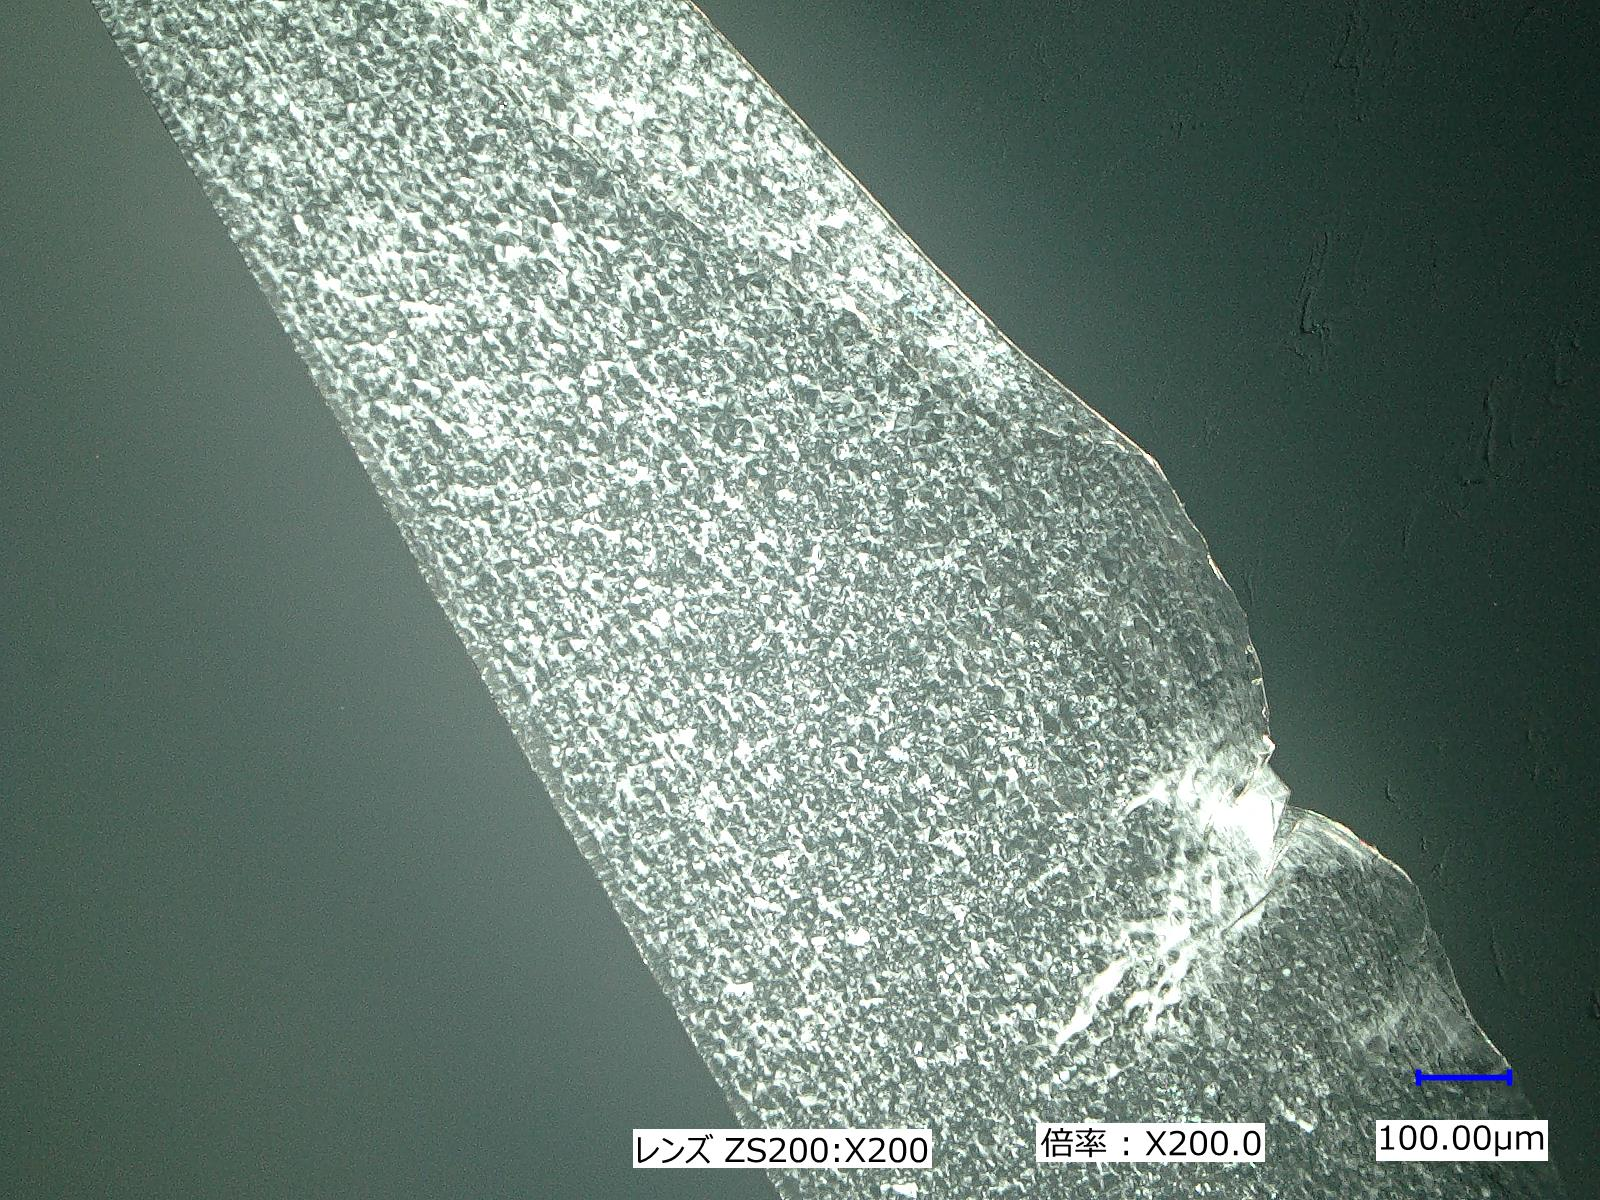
\includegraphics[keepaspectratio, scale=0.1]{Data/観察結果/rapid_cooling_200.jpg}
      \subcaption{Magnification 200x}
      \label{fig:rapid200}
    \end{minipage}
    \begin{minipage}[htbp]{0.45\linewidth}
      \centering
      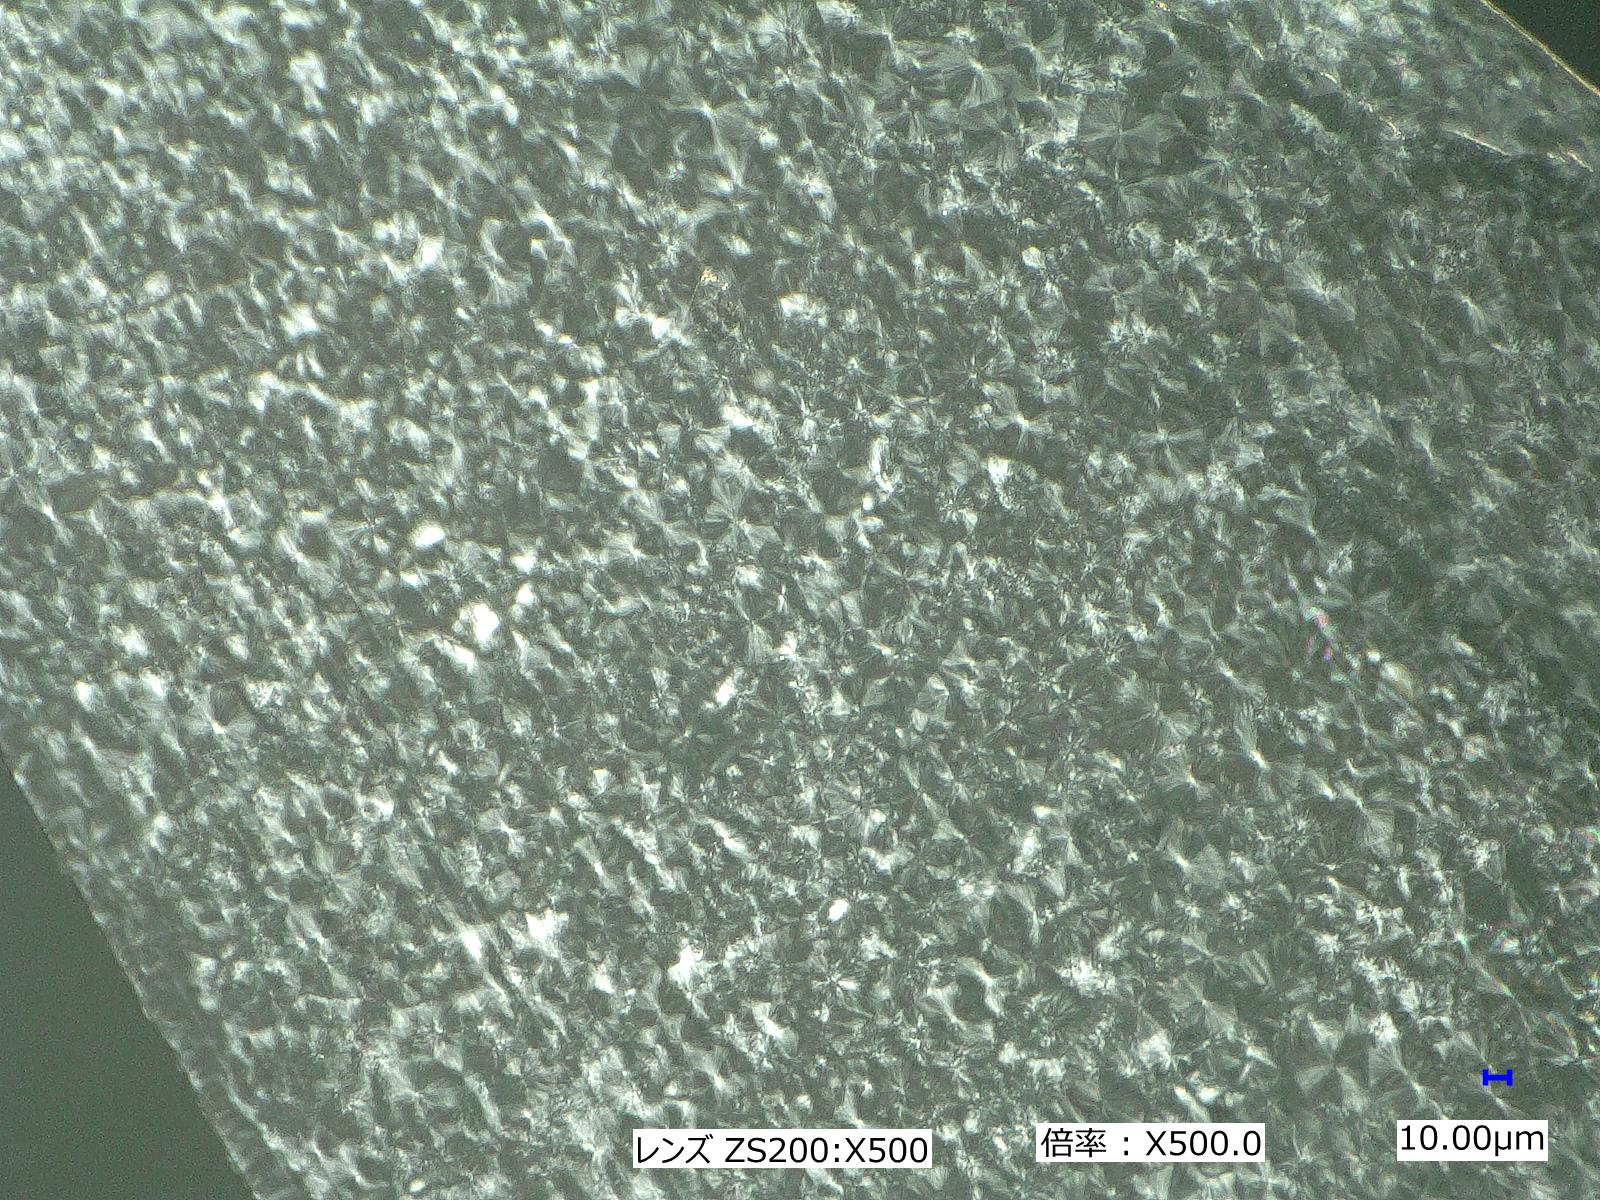
\includegraphics[keepaspectratio, scale=0.1]{Data/観察結果/rapid_cooling_500.jpg}
      \subcaption{Magnification 500x}
      \label{fig:rapid500}
    \end{minipage}
    \centering
    \caption{Rapidly cooled specimen.}
    \label{fig:rapid}
\end{figure}

\begin{figure}[htbp]
    \begin{minipage}[htbp]{0.45\linewidth}
      \centering
      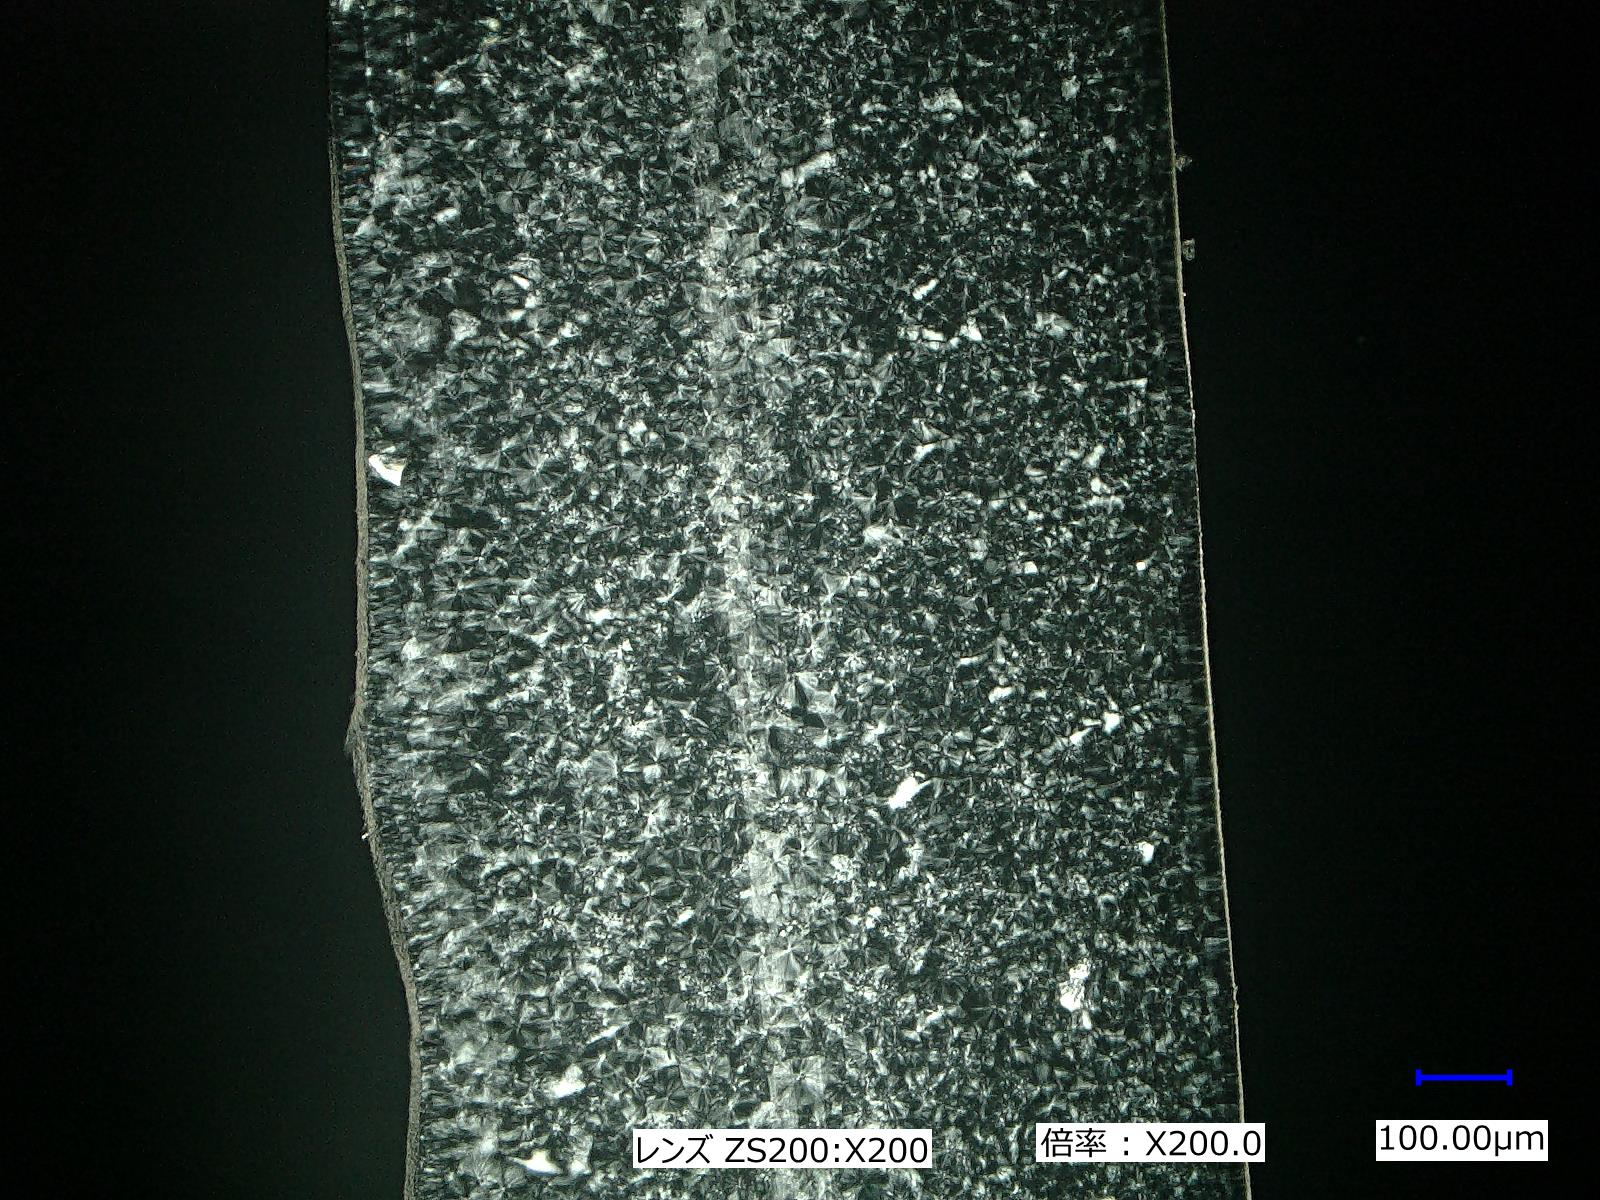
\includegraphics[keepaspectratio, scale=0.1]{Data/観察結果/65_10min_200.jpg}
      \subcaption{Magnification 200x}
      \label{fig:65度200}
    \end{minipage}
    \begin{minipage}[htbp]{0.45\linewidth}
      \centering
      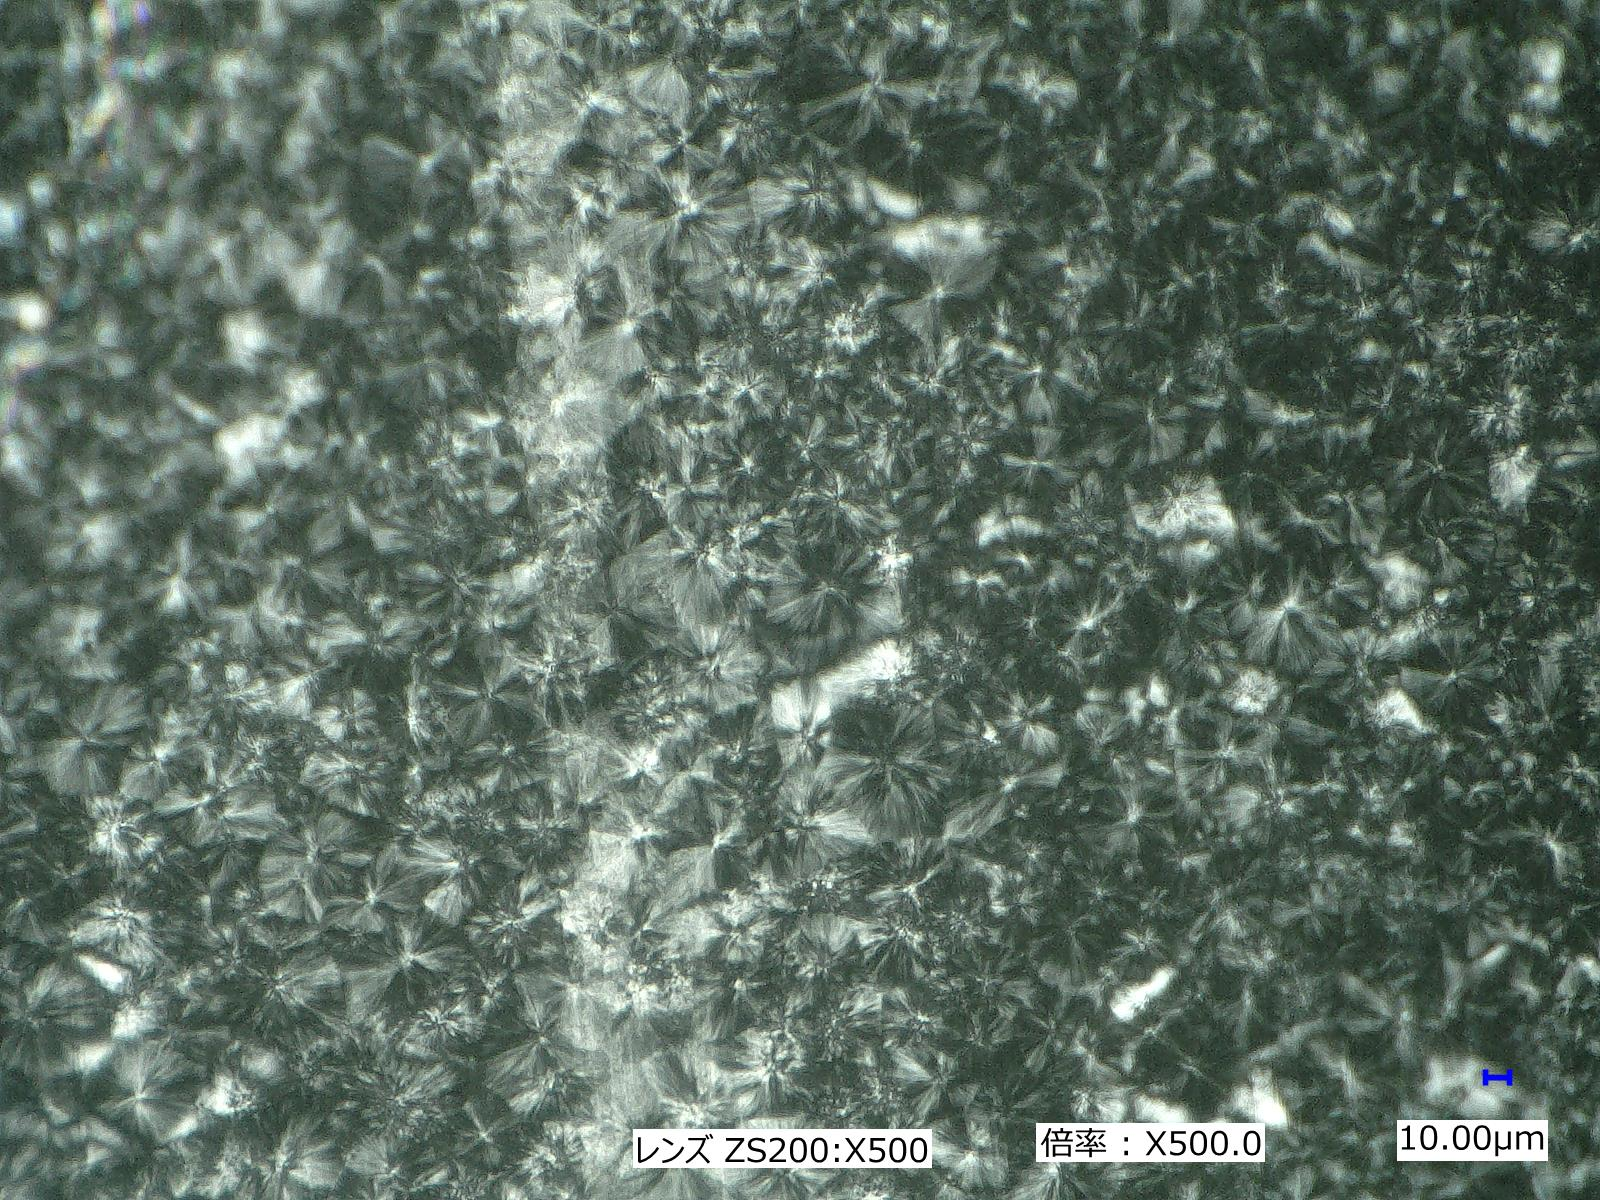
\includegraphics[keepaspectratio, scale=0.1]{Data/観察結果/65_10min_500.jpg}
      \subcaption{Magnification 500x}
      \label{fig:65度500}
    \end{minipage}
    \centering
    \caption{Specimen held at 65$^\circ$C for 10 minutes.}
    \label{fig:65度}
\end{figure}

\begin{figure}[htbp]
    \begin{minipage}[htbp]{0.45\linewidth}
      \centering
      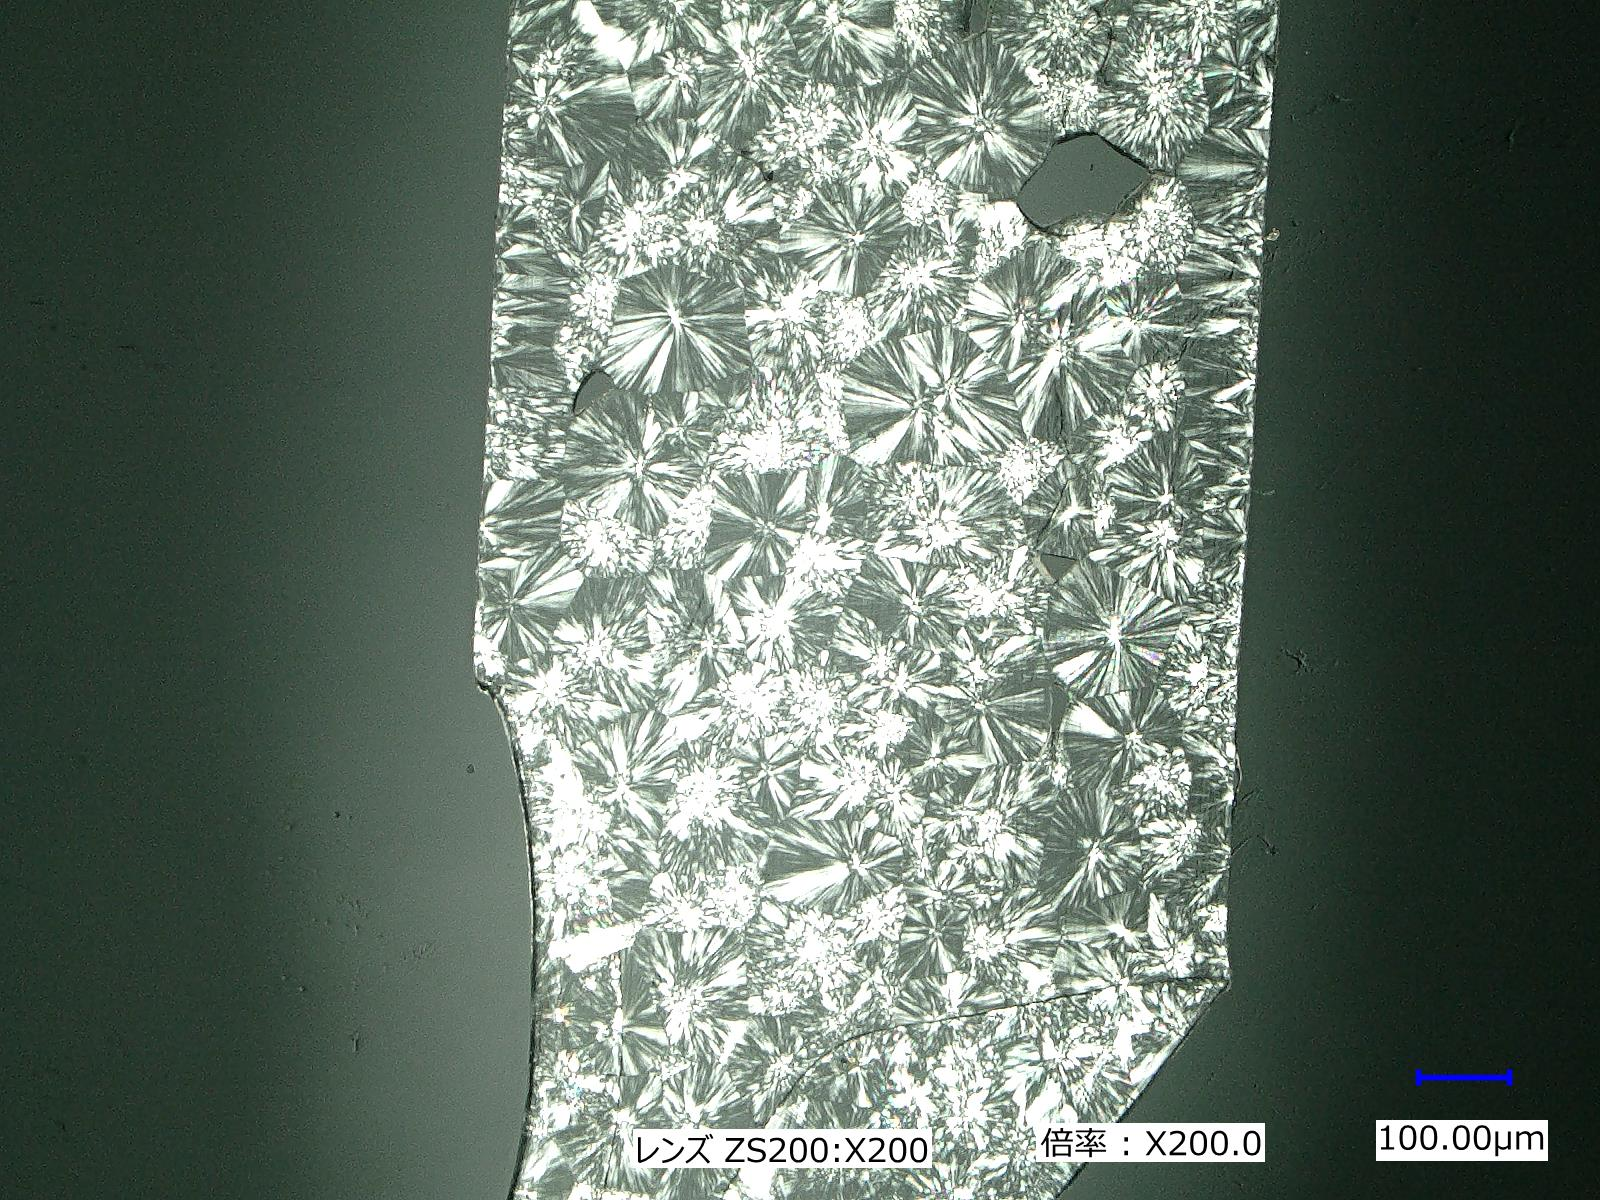
\includegraphics[keepaspectratio, scale=0.1]{Data/観察結果/120_10min_200.jpg}
      \subcaption{Magnification 200x}
      \label{fig:120度200}
    \end{minipage}
    \begin{minipage}[htbp]{0.45\linewidth}
      \centering
      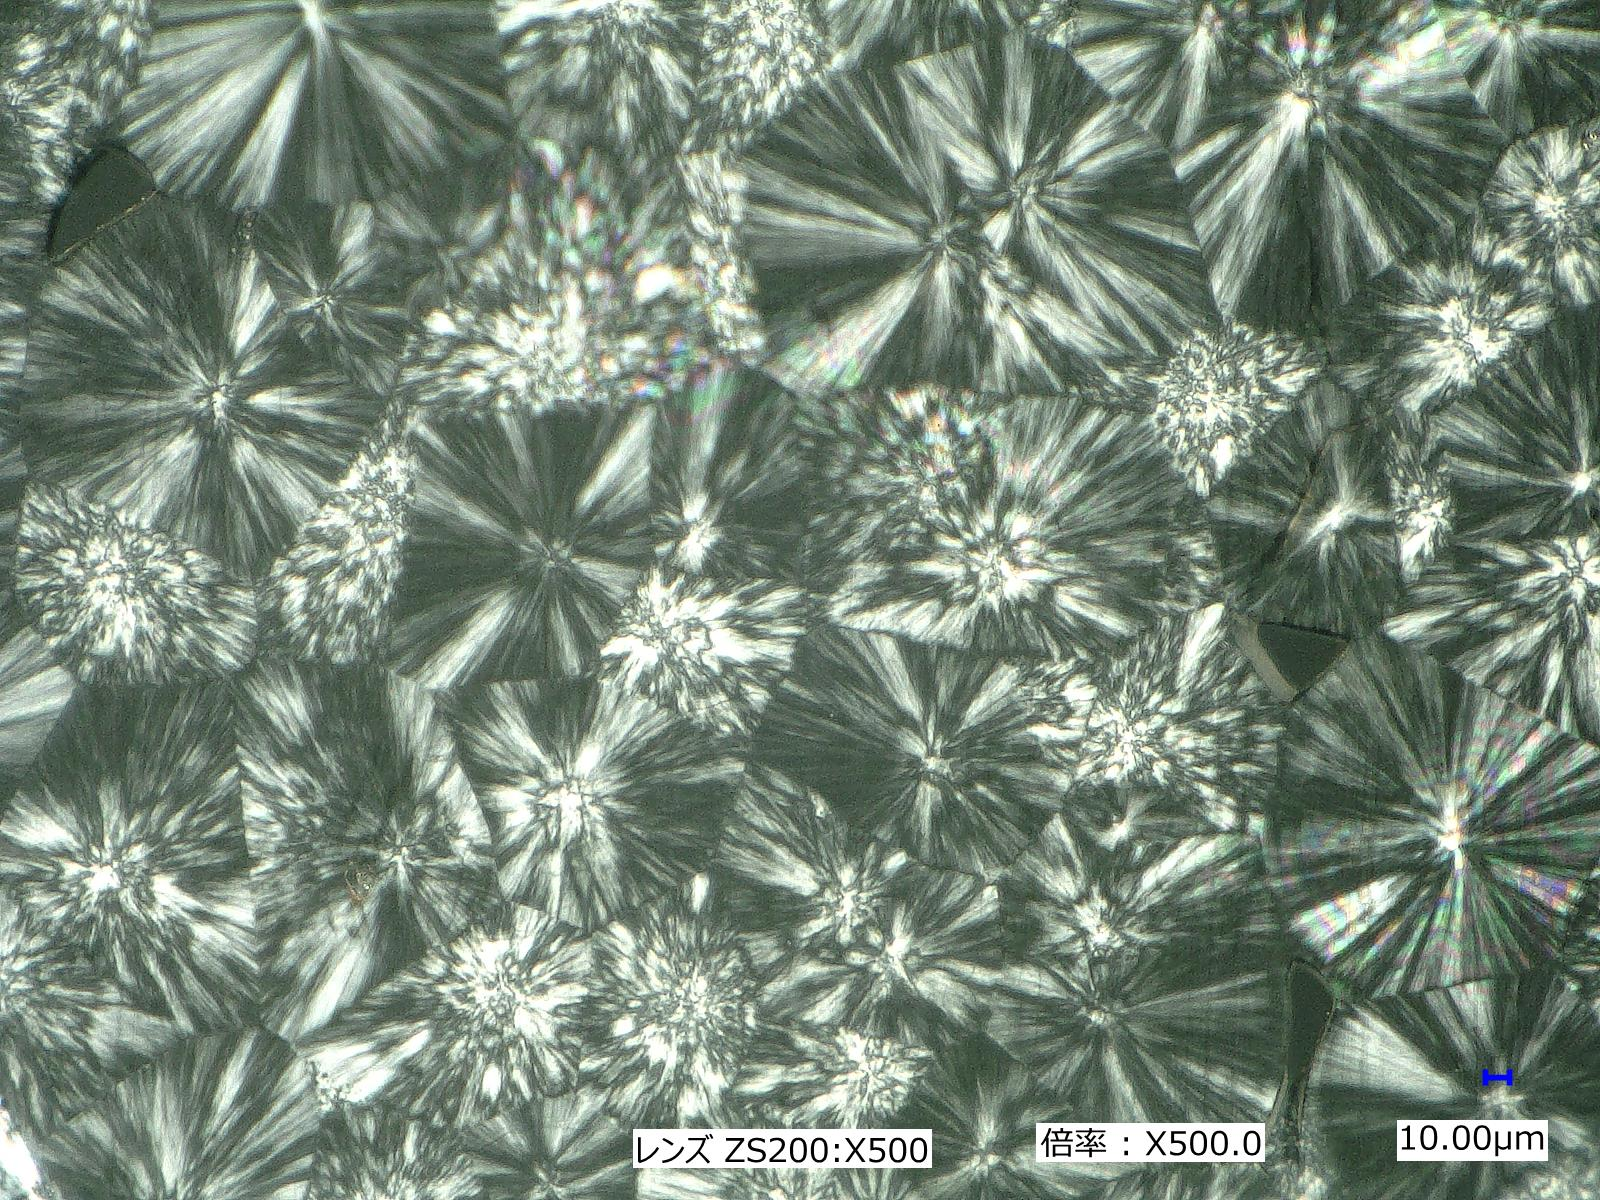
\includegraphics[keepaspectratio, scale=0.1]{Data/観察結果/120_10min_500.jpg}
      \subcaption{Magnification 500x}
      \label{fig:120度500}
    \end{minipage}
    \centering
    \caption{Specimen held at 120$^\circ$C for 10 minutes.}
    \label{fig:120度}
\end{figure}